\section{Bilanz und GuV im Accounting Equation Approach}

\textbf{Bilanz}: Momentaufnahme der wirtschaftlichen Situation eines Unternehmens zu einem bestimmten
Zeitpunkt
\begin{center}
	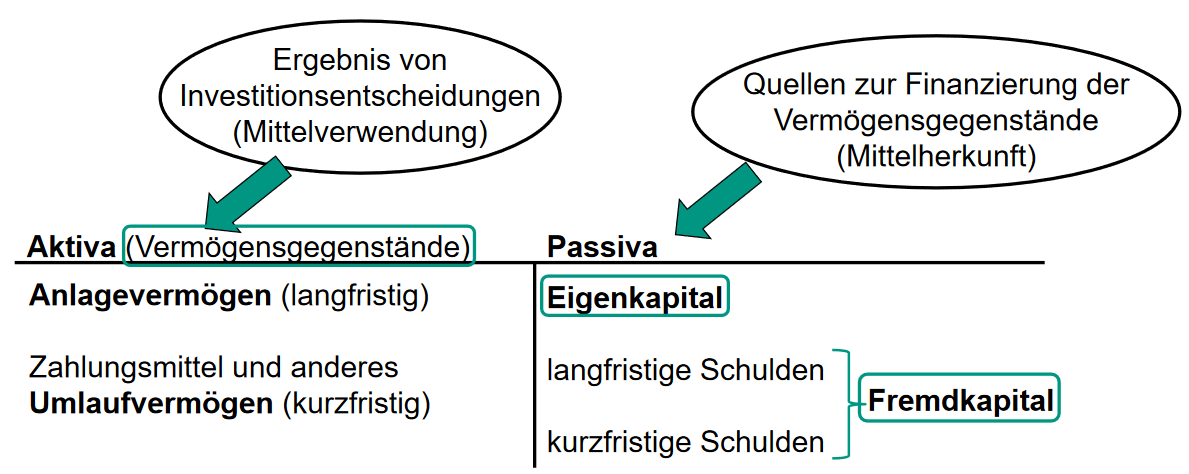
\includegraphics[width=0.7\textwidth]{images/bilanz.png}
\end{center}

\textbf{Vermögensgegenstände}: Repräsentieren zukünftige ökonomische Werte, die dem Unternehmen zufließen und zuverlässig in Geldeinheiten messbar sind
\begin{itemize}
	\item \textbf{Anlagevermögen} (langfristig): Sachanlagen, Finanzanlagen, Immaterielle Vermögensgegenstände, Aktive latente Steuern
	\item \textbf{Umlaufvermögen} (kurzfristig): Vorräte, Geleistete Anzahlungen, Forderungen, Wertpapiere, Liquide Mittel
	\item Vermögensgegenstände oft nur zu historischen Anschaffungskosten bewertet oder noch niedriger (Abschreibungen)
	\item Wertvolle Unternehmenseigenschaften, wie z.B. Humankapital (Fähigkeiten und Erfahrung der Mitarbeiter), Verträge über Großaufträge, Reputation und Marke bleiben unberücksichtigt!
	$\rightarrow$ Vorsichtsprinzip
\end{itemize}
\pagebreak
\textbf{Fremdkapital}: \textbf{Schulden}, d.h. Verpflichtungen des Unternehmens um Geld, Güter und Dienstleistungen an einen externen Anspruchsberechtigten bereitzustellen, die zuverlässig in Geldeinheiten messbar sind.
Beispiele:
\begin{itemize}
	\item Verbindlichkeiten, z.B. Kredit, Verpflichtungen, Steuern, Höhe und Fälligkeit stehen fest
	\item Rückstellungen, z.B. Pensionen, Höhe und Fälligkeit werden geschätzt
	\item Muss auf dem Matching Principle genügen!
\end{itemize}
\bigskip
\textbf{Eigenkapital}: Reinvermögen des Unternehmens (= Wert der Vermögensgegenstände $-$ Wert der Schulden) und entspricht dem Unternehmenswert aus Perspektive der Eigentümer.
Besteht aus:
\begin{itemize}
	\item Gezeichnetes Kapital $+$ Kapitalrücklage $\rightarrow$ eingezahlt von den Gesellschaftern
	\item Gewinnrücklage $\rightarrow$ kumuliert aus bisherigen Gewinnen
\end{itemize}
\bigskip

\begin{wrapfigure}{r}{4.5cm}
	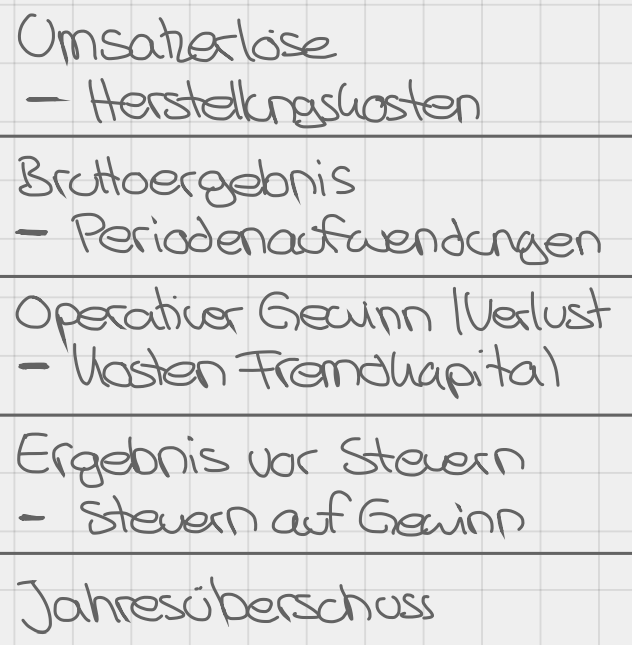
\includegraphics[width=0.3\textwidth]{images/guv-ex.png}
	\vspace{-100pt}
\end{wrapfigure} 

\textbf{Gewinn- und Verlustrechnung (GuV)}:
\begin{itemize}
	\item Wirtschaftlicher Erfolg = Umsatzerlöse (Realisationsprinzip) $-$ Aufwendungen (Matching Principle)
	\item Zwei Arten von Aufwendungen:
	\begin{itemize}
		\item Herstellungskosten (sachliche Abgrenzung)
		\item Periodenaufwendungen (zeitliche Abgrenzung)
	\end{itemize}
	\item Nur Veränderungen des EK aus gewöhnlichen\\ Geschäftstätigkeiten gehen in die GuV ein!\\
	Interaktionen mit Eigentümern, wie z.B. Dividendenauszahlung irrelevant.
\end{itemize}
\bigskip
\textbf{Grundformen der Verbuchung}:
\begin{itemize}
	\item \textbf{Antizipative Rechnungsabgrenzung}: Vorwegnahme von Aufwendungen wofür Zahlungen erst in einer späteren Periode erfolgen (3 und 5).
	\item \textbf{Transitorische Rechnungsabgrenzung}: Aufwendungen und Umsatzerlöse in nächste Periode übertragen, obwohl Zahlungen bereits erfolgt (2 und 6).
\end{itemize}
\begin{center}
	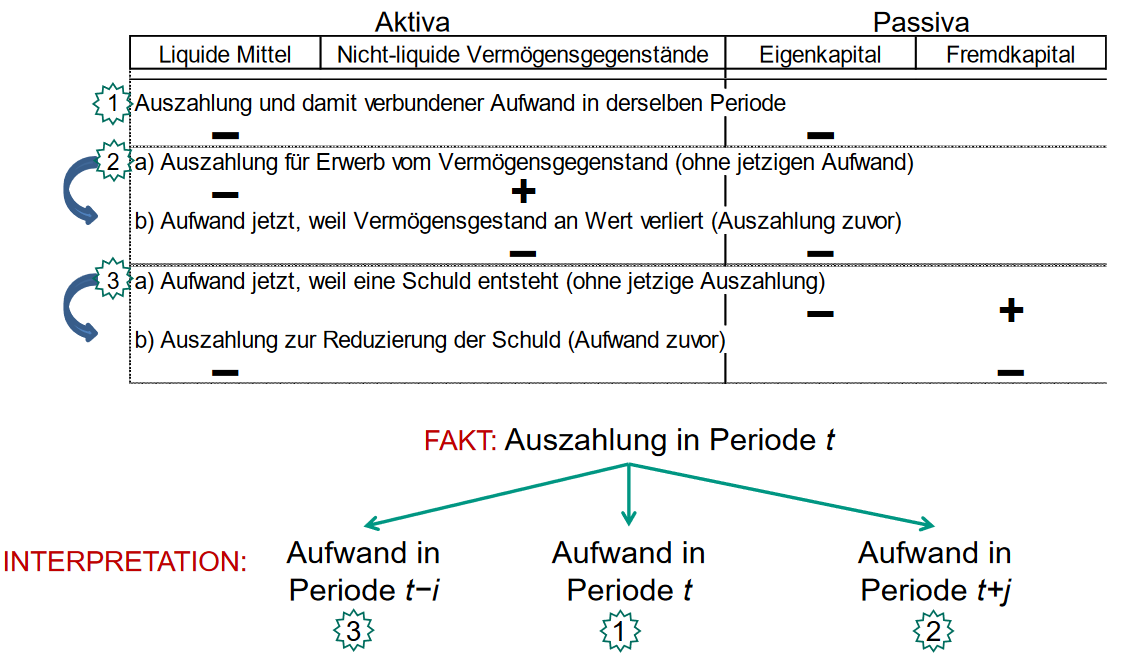
\includegraphics[width=0.8\textwidth]{images/gf1.png}
\end{center}
\begin{center}
	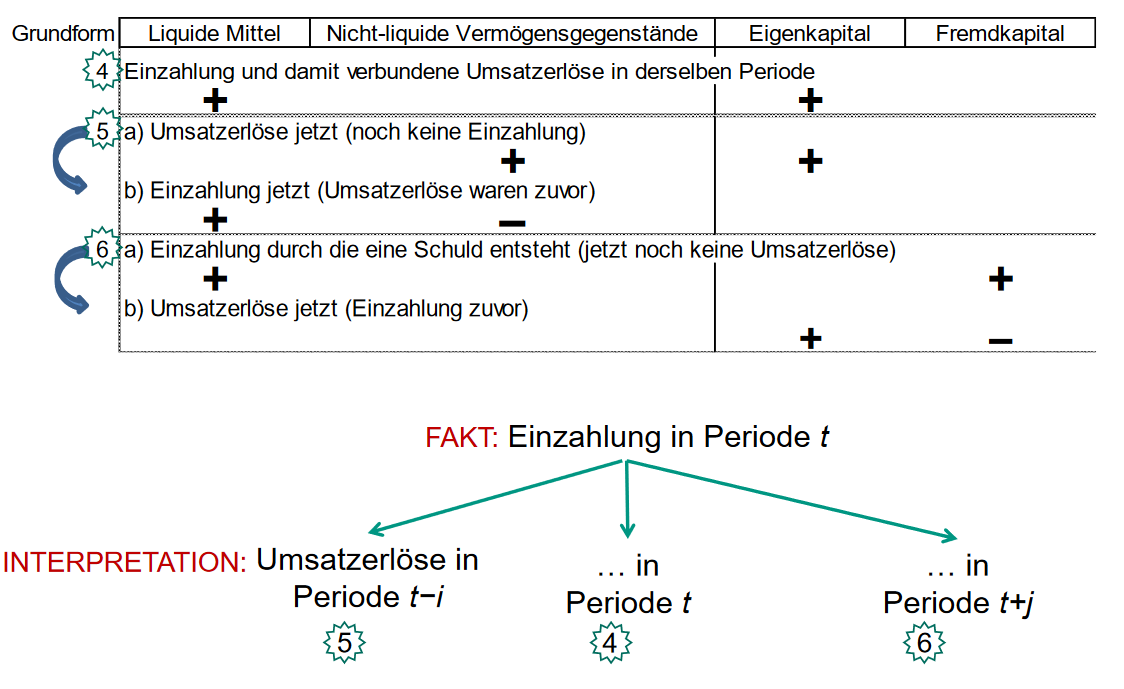
\includegraphics[width=0.8\textwidth]{images/gf2.png}
\end{center}

\textbf{Worksheet Approach} Bilanz und GuV: s. FS2/21-28, \underline{ÜBEN}!
\begin{itemize}
	\item Erste Zeile Bilanz: \textbf{Eröffnungsbilanz}, Erste Zeile GuV: leer
	\item $\text{Gewinn}=\text{EK}_\text{Schlussbilanz}–\text{EK}_\text{Eröffnungsbilanz}$
	\item Für jeden Geschäftsvorfall gilt:
	\begin{itemize}
		\item $\Delta L + \Delta V=\Delta E+\Delta F$ \\
		$L$: Liquide Mittel, $V$: Nicht-liquide Vermögensgegenstände, $E$: EK, $F$: FK
		\item $\Delta E=U-A$\\
		$U$: Umsatzerlöse, $A$: Aufwendungen
		\item Passiva und Aktiva gleich verändert
	\end{itemize}
\end{itemize}
\begin{center}
	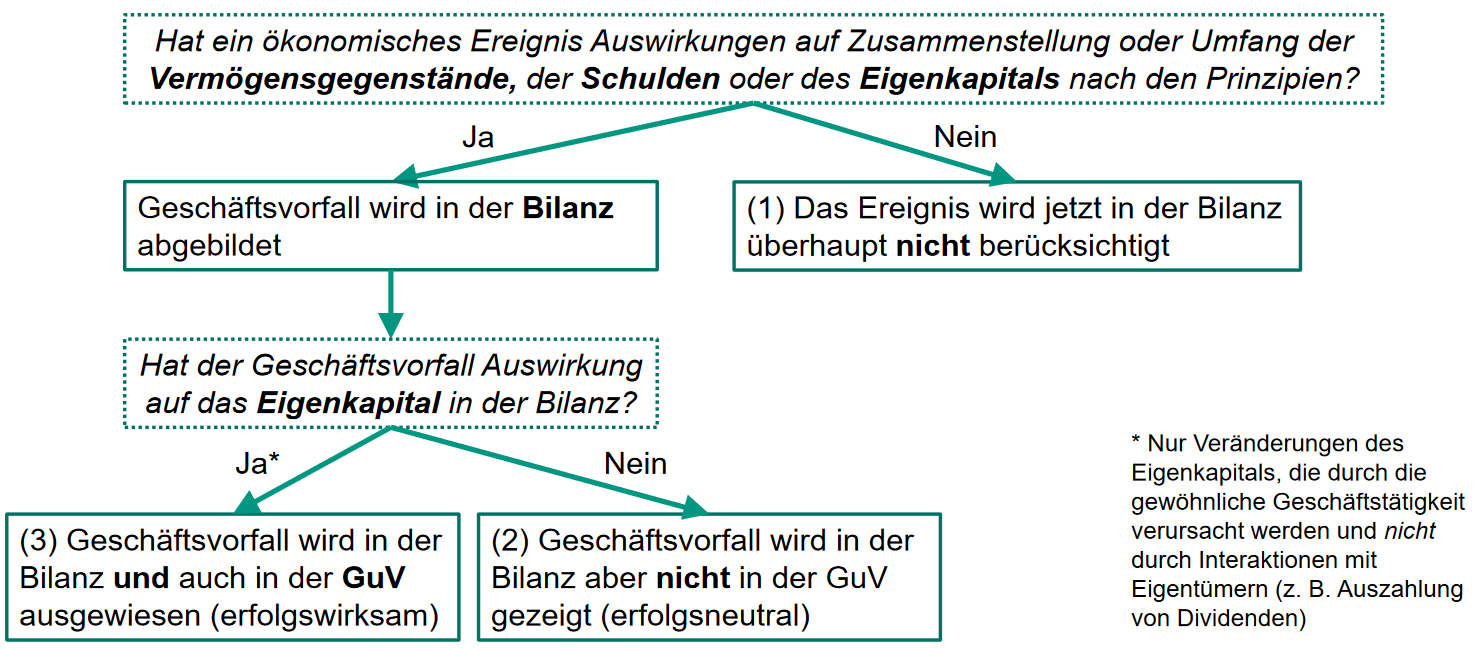
\includegraphics[width=0.8\textwidth]{images/sze.png}
\end{center}
\textbf{Häufige Geschäftsvorfälle}:
\begin{center}
	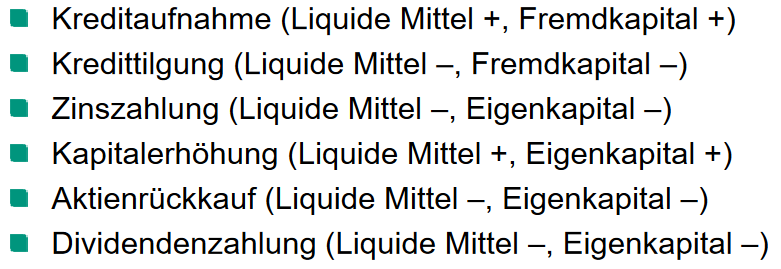
\includegraphics[width=0.5\textwidth]{images/gsv.png}
\end{center}
\bigskip

\textbf{T-Konten}: